\subsection{Plane strain bracket}
\paragraph{}
In this example, a plane strain bracket with a downward uniform distributed load on the top is considered (see fig.~\ref{qdt_fig:ex_bracket_geo_bc}).
The material properties are: Young’s modulus $E = 2\times 10^5 N/m^2$ and Poisson’s ratio $\nu = 0.3$.
    \begin{figure}[H]
        \centering
        \begin{subfigure}[b]{1\linewidth}
            \centering
            \scalebox{1.2}{
                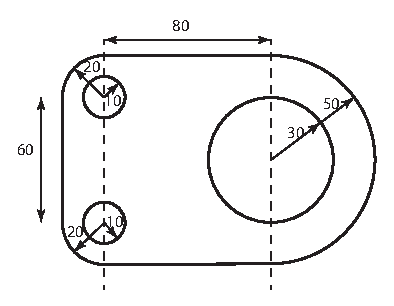
\includegraphics{quadtree/ex_images/ex_bracket_geo.eps}
            }
        \end{subfigure}
        \begin{subfigure}[b]{1\linewidth}
            \centering
            \scalebox{1.3}{
                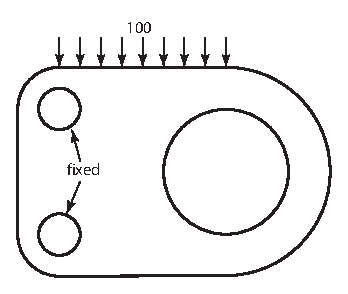
\includegraphics{quadtree/ex_images/ex_bracket_load.eps}
            }
        \end{subfigure}
        \caption{ Plane strain bracket: geometry and boundary conditions}
        \label{qdt_fig:ex_bracket_geo_bc}
    \end{figure}

\paragraph{}
A total strain energy of $282.927$ is determined by ANSYS with the mesh shown in fig.~\ref{qdt_fig:ex_bracket_ansys_mesh}
    \begin{figure}[H]
        \centering
        \scalebox{0.35}{
            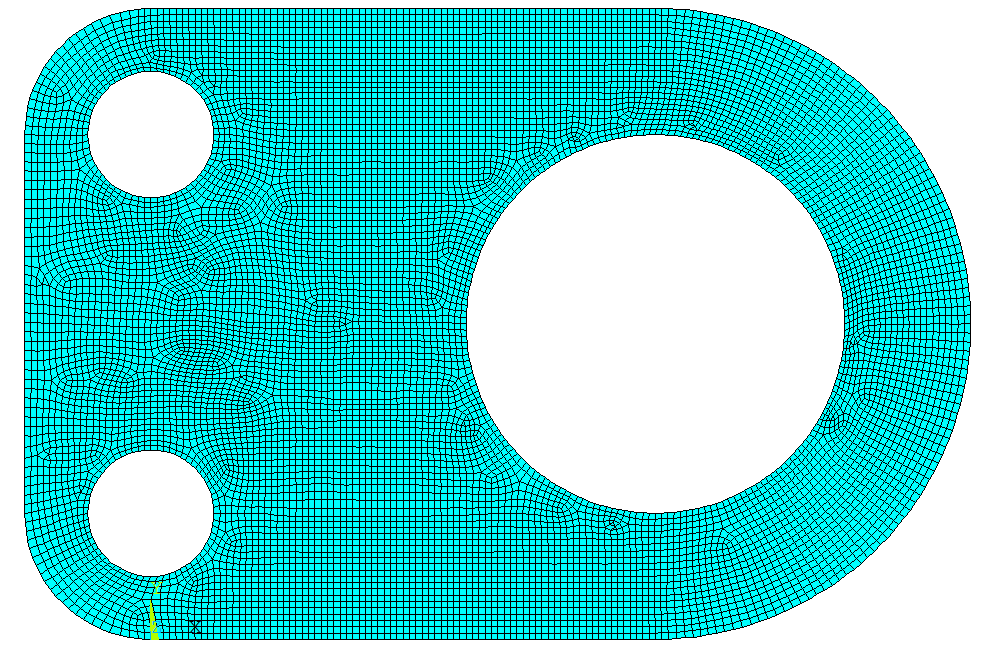
\includegraphics{quadtree/ex_images/ex_bracket_ansys_mesh_31002nodes.png}
        }
        \caption{ANSYS mesh for plane strain bracket (62004 DOF)}
        \label{qdt_fig:ex_bracket_ansys_mesh}
    \end{figure}

\paragraph{}
Drawing in AutoCAD will be divided into two parts: base and the holes as shown in fig.~\ref{qdt_fig:ex_bracket_cad}
    \begin{figure}[H]
        \centering
        \begin{subfigure}[b]{1\linewidth}
            \centering
            \scalebox{0.4}{
                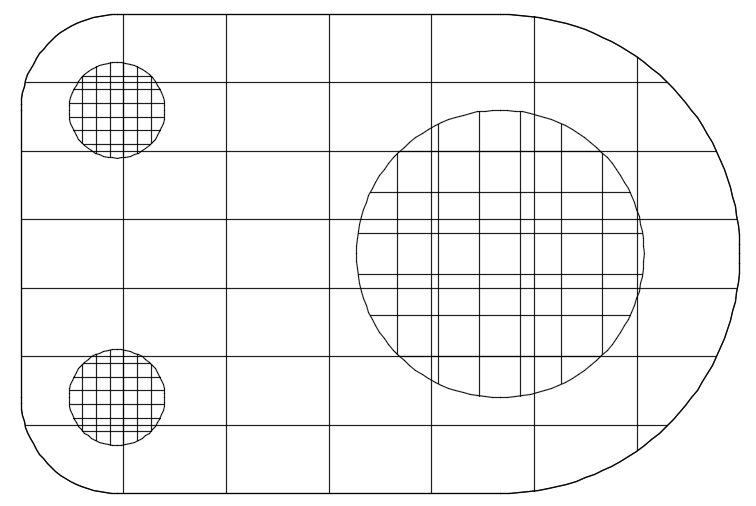
\includegraphics{quadtree/ex_images/ex_bracket_cad_full.png}
            }
            \caption{All}
        \end{subfigure}
        \begin{subfigure}[b]{0.4\linewidth}
            \scalebox{0.2}{
                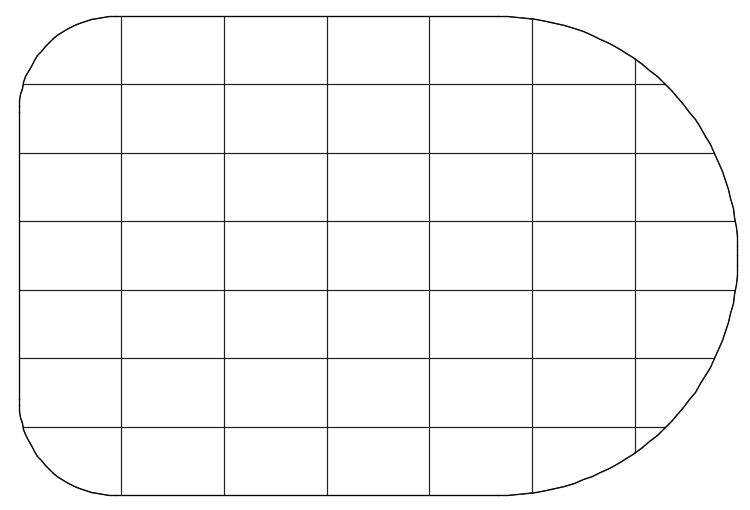
\includegraphics{quadtree/ex_images/ex_bracket_cad_base.png}
            }
            \caption{Base}
        \end{subfigure}
        \begin{subfigure}[b]{0.4\linewidth}
            \scalebox{0.2}{
                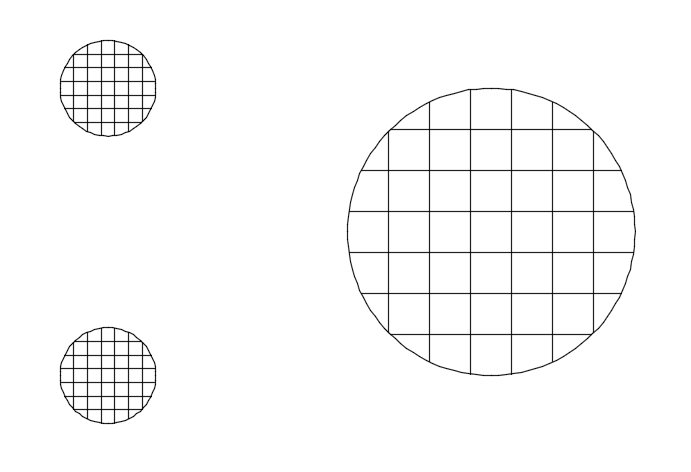
\includegraphics{quadtree/ex_images/ex_bracket_cad_holes.png}
            }
            \caption{Holes}
        \end{subfigure}
        \caption{CAD drawing of plane strain bracket}
        \label{qdt_fig:ex_bracket_cad}
    \end{figure}
% fig- 64,32/8,3
Generated background mesh, coloring and the final result with $res=32$, $s_{max}=4$ and $s_{min}=1$ are shown in fig.~\ref{qdt_fig:ex_chole_background_mesh}, fig.~\ref{qdt_fig:ex_chole_mesh_coloring} and fig.~\ref{qdt_fig:ex_chole_mesh_final}.
\begin{figure}
    \centering
    \scalebox{0.4}{
        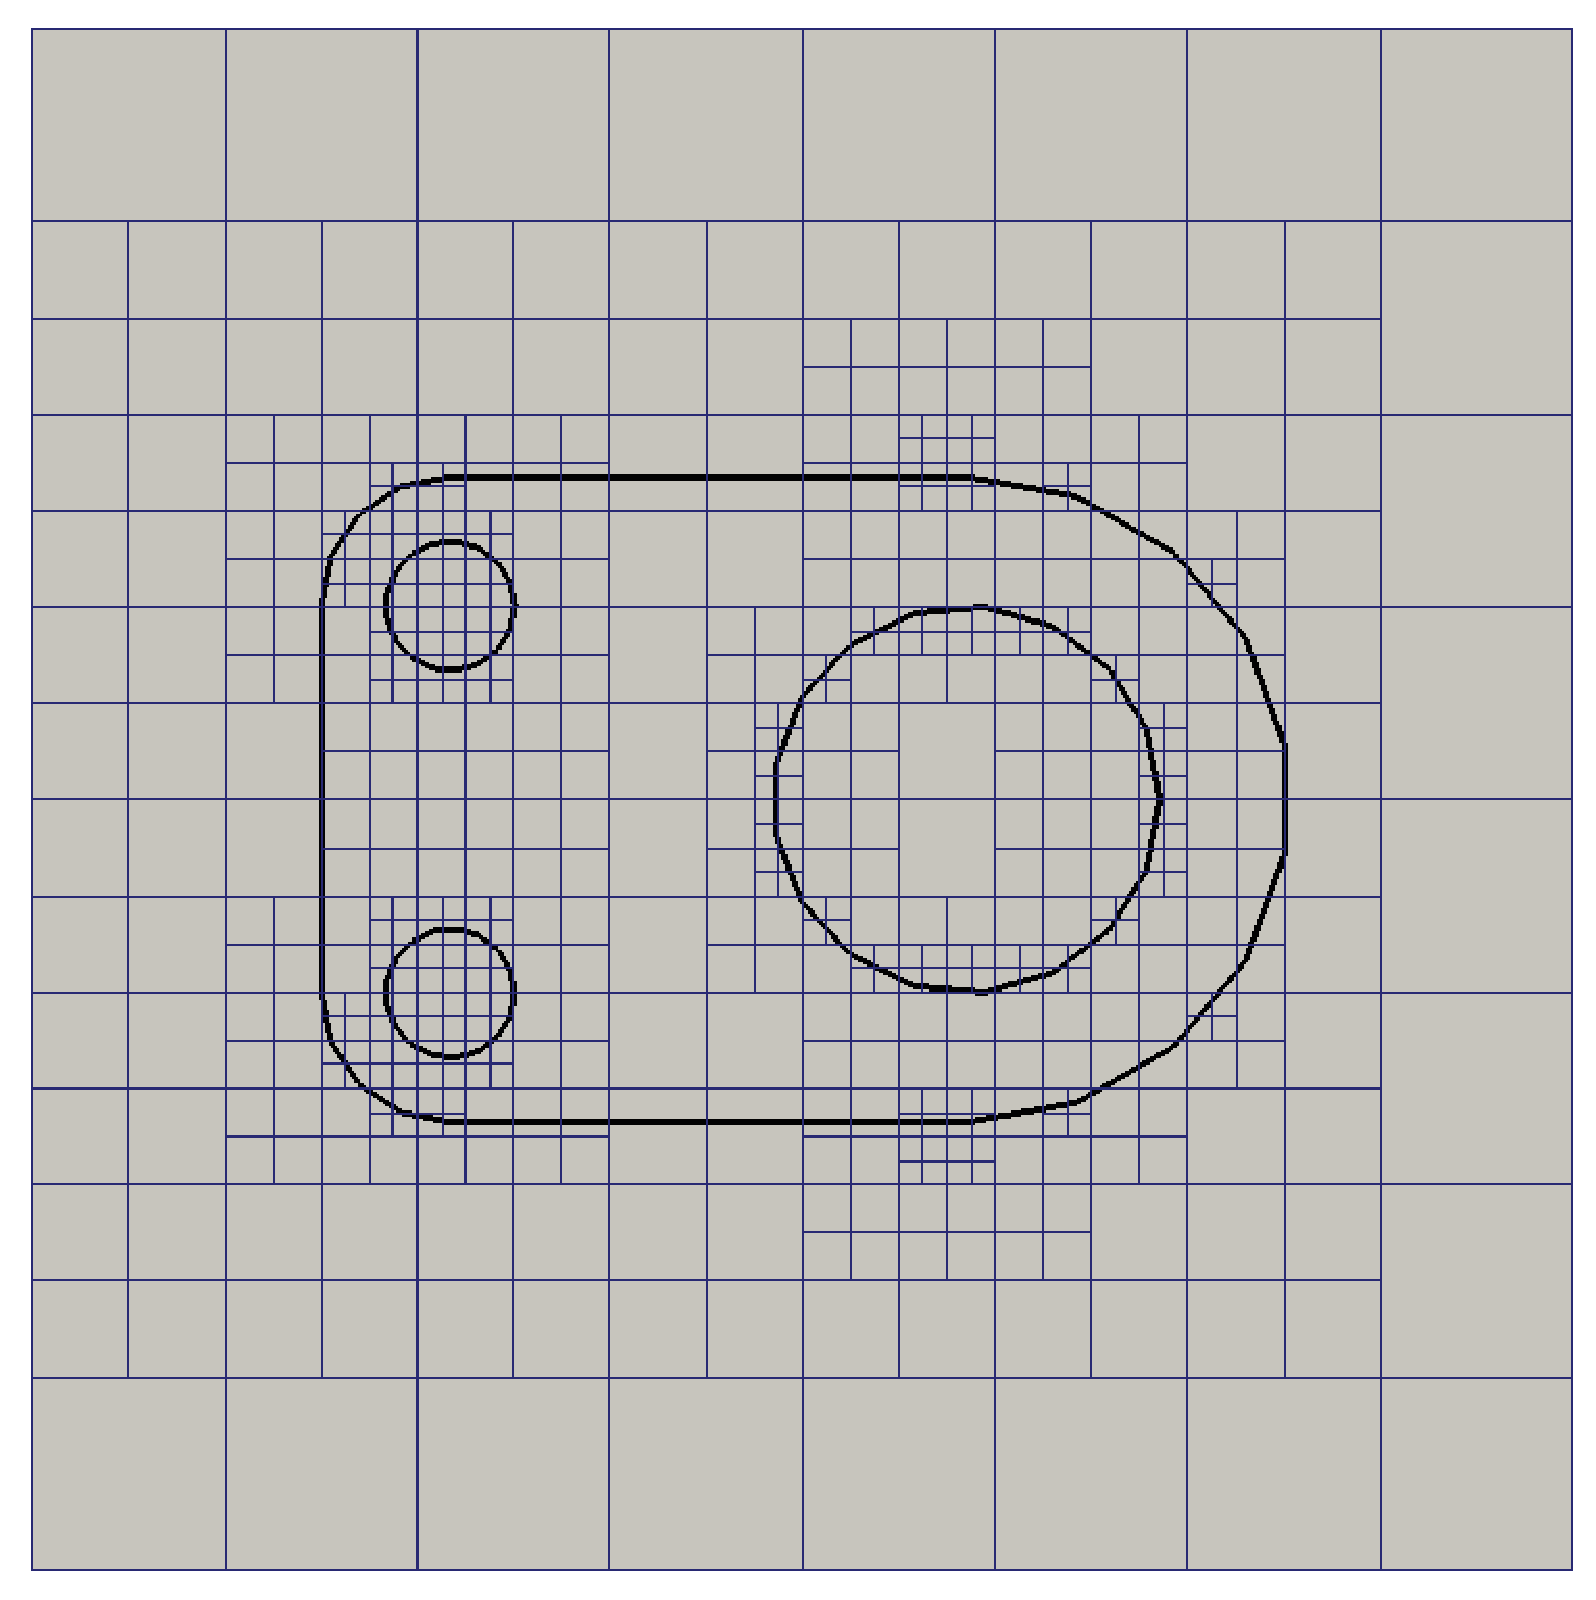
\includegraphics{quadtree/ex_images/ex_bracket_background.eps}
    }
    \caption[Background mesh of the bracket]{Background mesh of the bracket : Bold lines represents the input geometry}
    \label{qdt_fig:ex_chole_background_mesh}
\end{figure}

\begin{figure}
    \centering
    \scalebox{0.5}{
        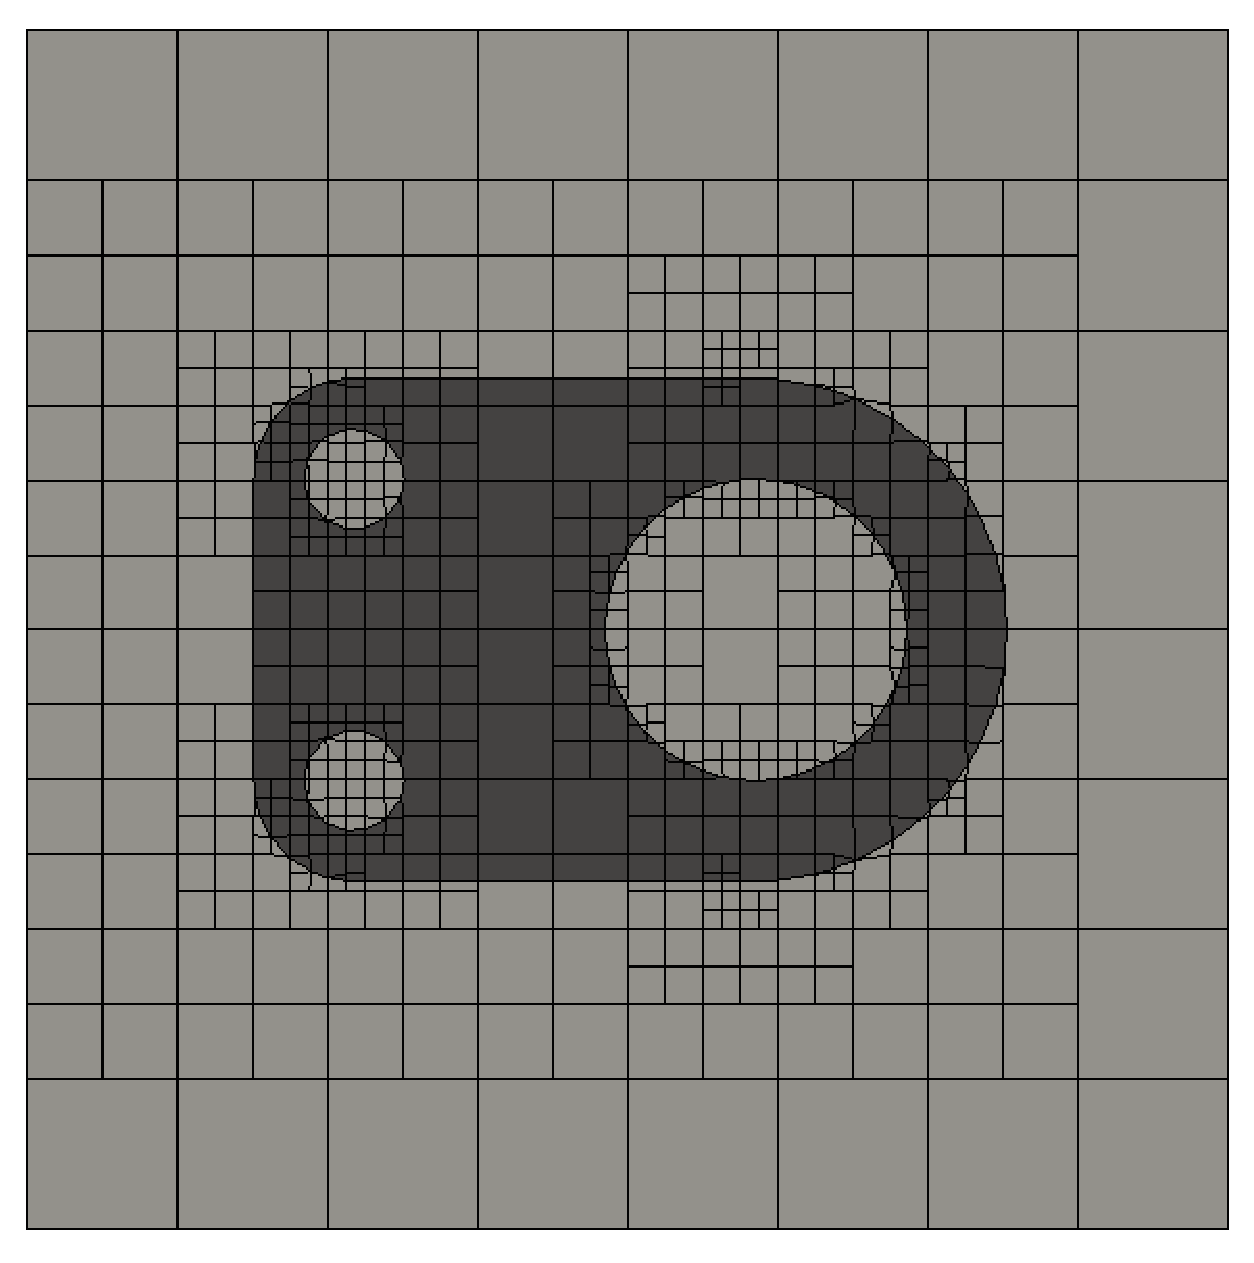
\includegraphics{quadtree/ex_images/ex_bracket_colored.eps}
    }
    \caption[Mesh coloring of the bracket]{Mesh coloring of the bracket : Grey area represents the bracket}
    \label{qdt_fig:ex_chole_mesh_coloring}
\end{figure}

\begin{figure}
    \centering
    \scalebox{0.3}{
        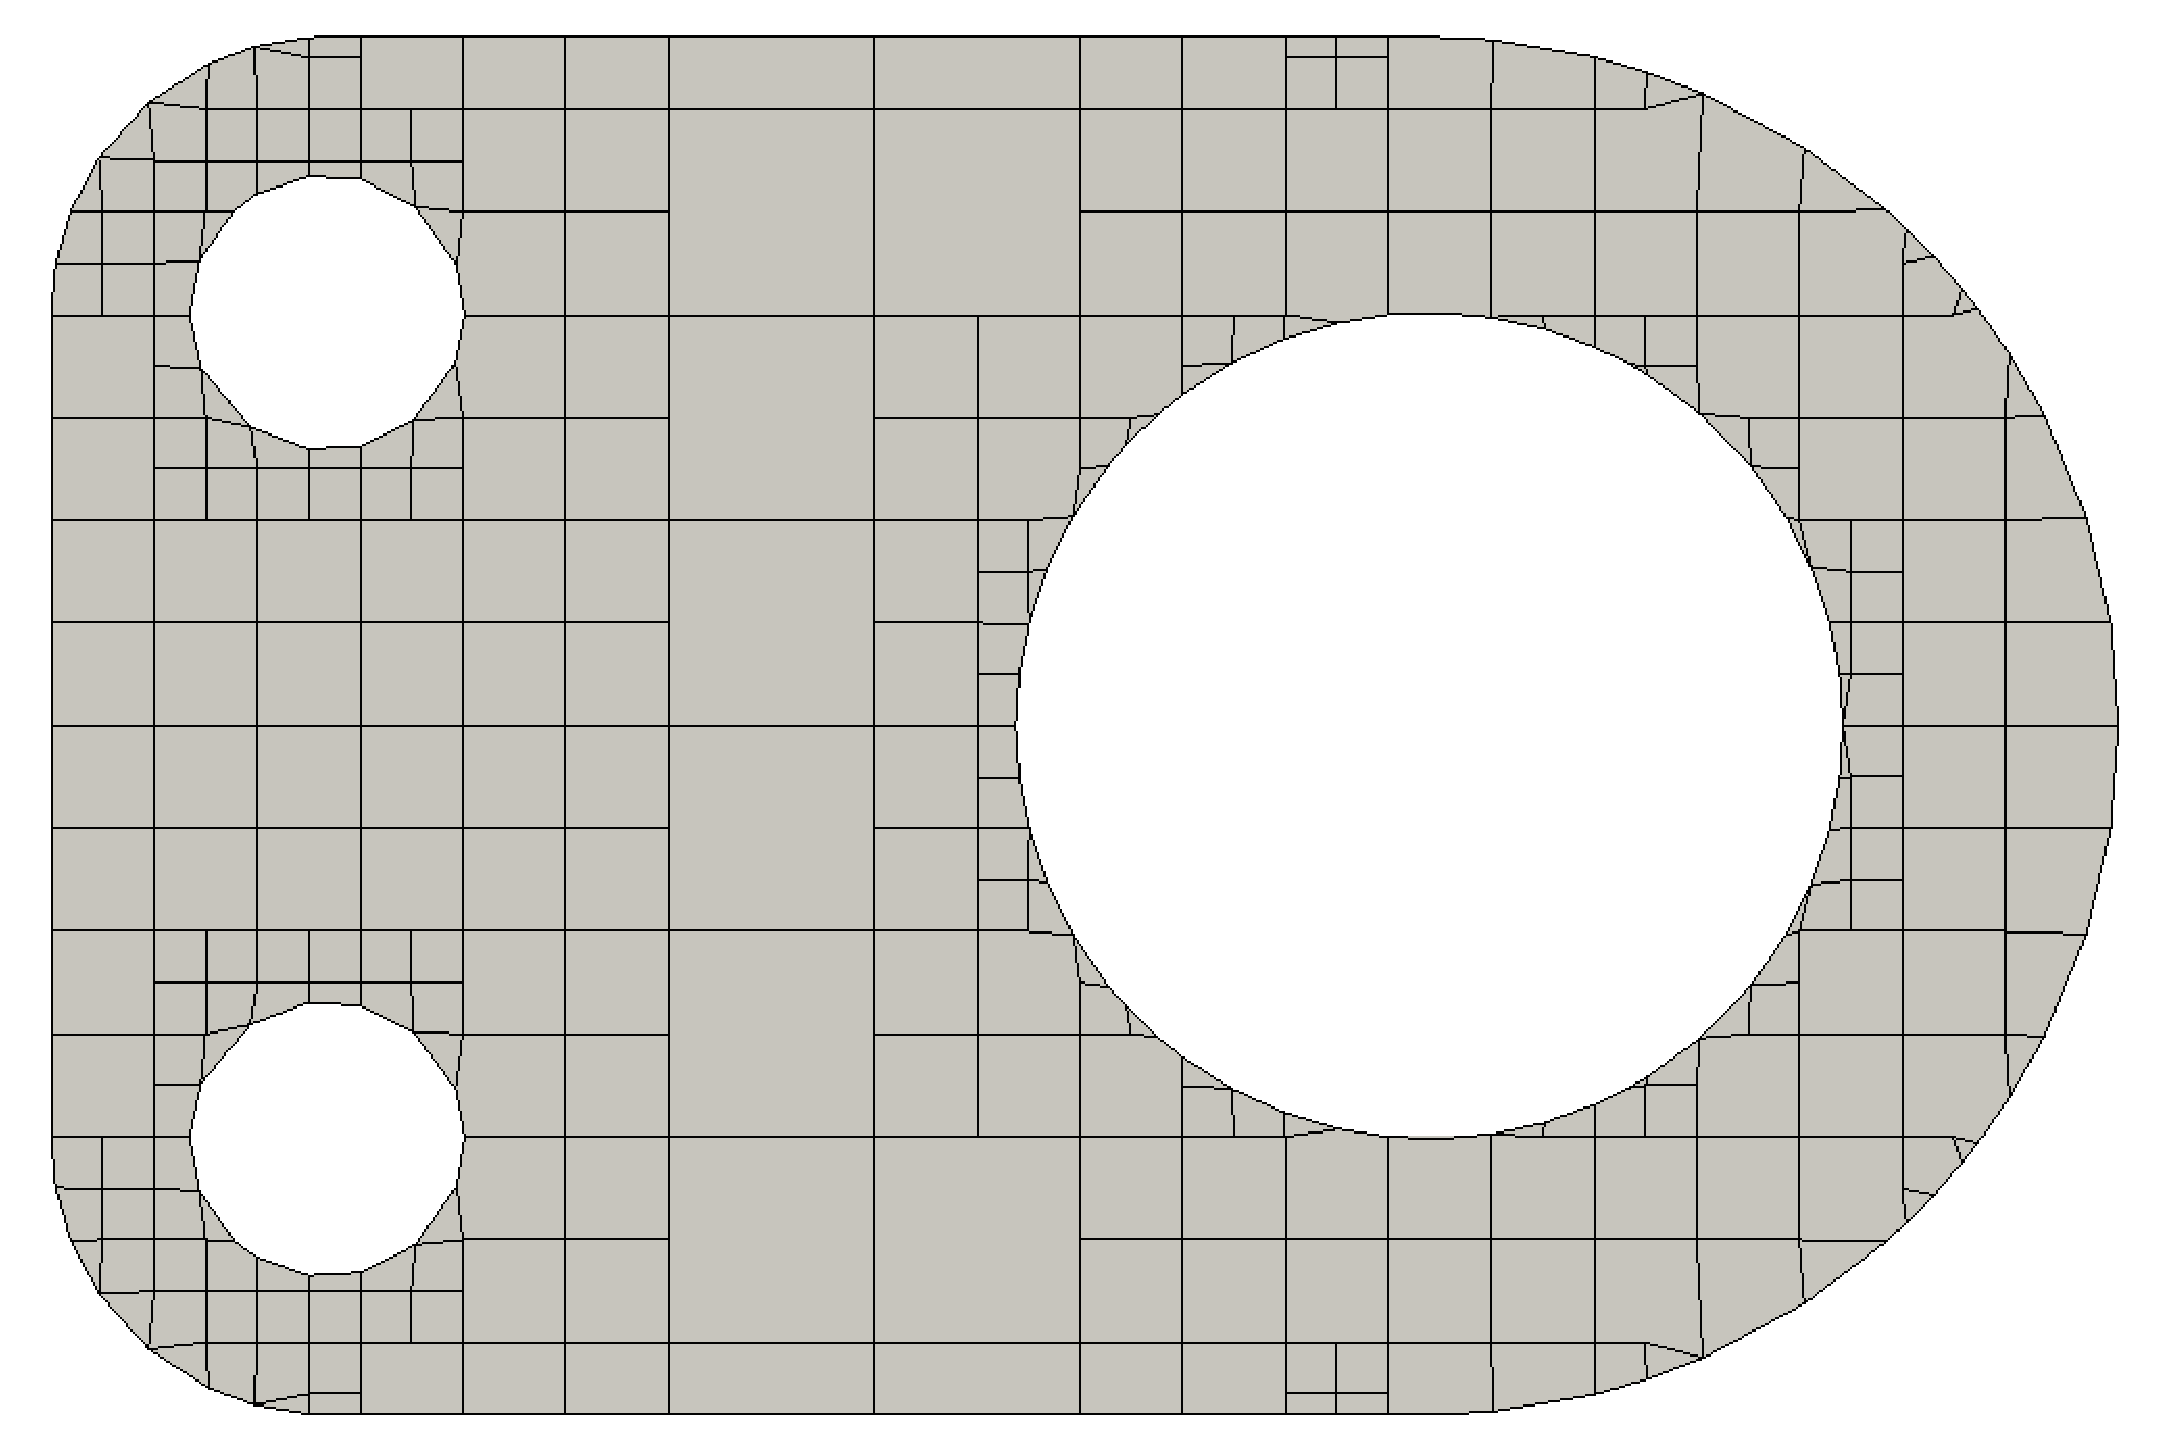
\includegraphics{quadtree/ex_images/ex_bracket_final.eps}
    }
    \caption[Final mesh of the bracket]{Final mesh of the bracket}
    \label{qdt_fig:ex_chole_mesh_final}
\end{figure}
% -1 - 282.927
% 382*2  - 274.5638 (32-4/8-3)
% 950*2  - 280.1255 (64-4/8-3)
% 2110*2 - 281.0799 (128-4/15-4)
% 4414*2 - 282.0363 (256-4/15-4)


% mlp
% 530 - 279.8076
% 1554 - 282.0745
% 4208 - 282.6581
% err = abs([279.8076 ,282.0745,282.6581]-282.927)/282.927; dof = [530,1554,4208]; polyfit(log(dof),log(err),1)

% uniform
% 530 - 279.8076
% 1810 - 282.3186
% 6464 - 282.674
% err_un = abs([279.8076 ,282.3186 ,282.674]-282.927)/282.927; dof_un = [530,1810,6464]; polyfit(log(dof_un),log(err_un),1)

% ansys-2nd
% 406*2 -  282.412
% 1144*2 - 282.895
% 4270*2 - 282.923

% 16462*2 -  282.926
% err_a2 = abs([282.412,282.895,282.923]-282.927)/282.927; dof_a2 = [406,1144,4270]*2; polyfit(log(dof_a2),log(err_a2),1)

% ansys-1st
% 185*2 - 275.635    
% 650*2 -  280.006   
% 1227*2 -  281.502 
% 2405*2 - 282.136
% err_a1 = abs([275.635,280.006  ,281.502 ,282.136]-282.927)/282.927; dof_a1 = [185,650,1227,2405]*2; polyfit(log(dof_a1),log(err_a1),1)
Mesh with different parameters are plotted in fig.~\ref{qdt_fig:ex_bracket_mesh_all} and the convergence study is plotted in fig.~\ref{qdt_fig:ex_bracket_mesh_conv}

\begin{figure}[H]
    \begin{subfigure}[b]{1\linewidth}
        \centering
        \scalebox{0.4}{
            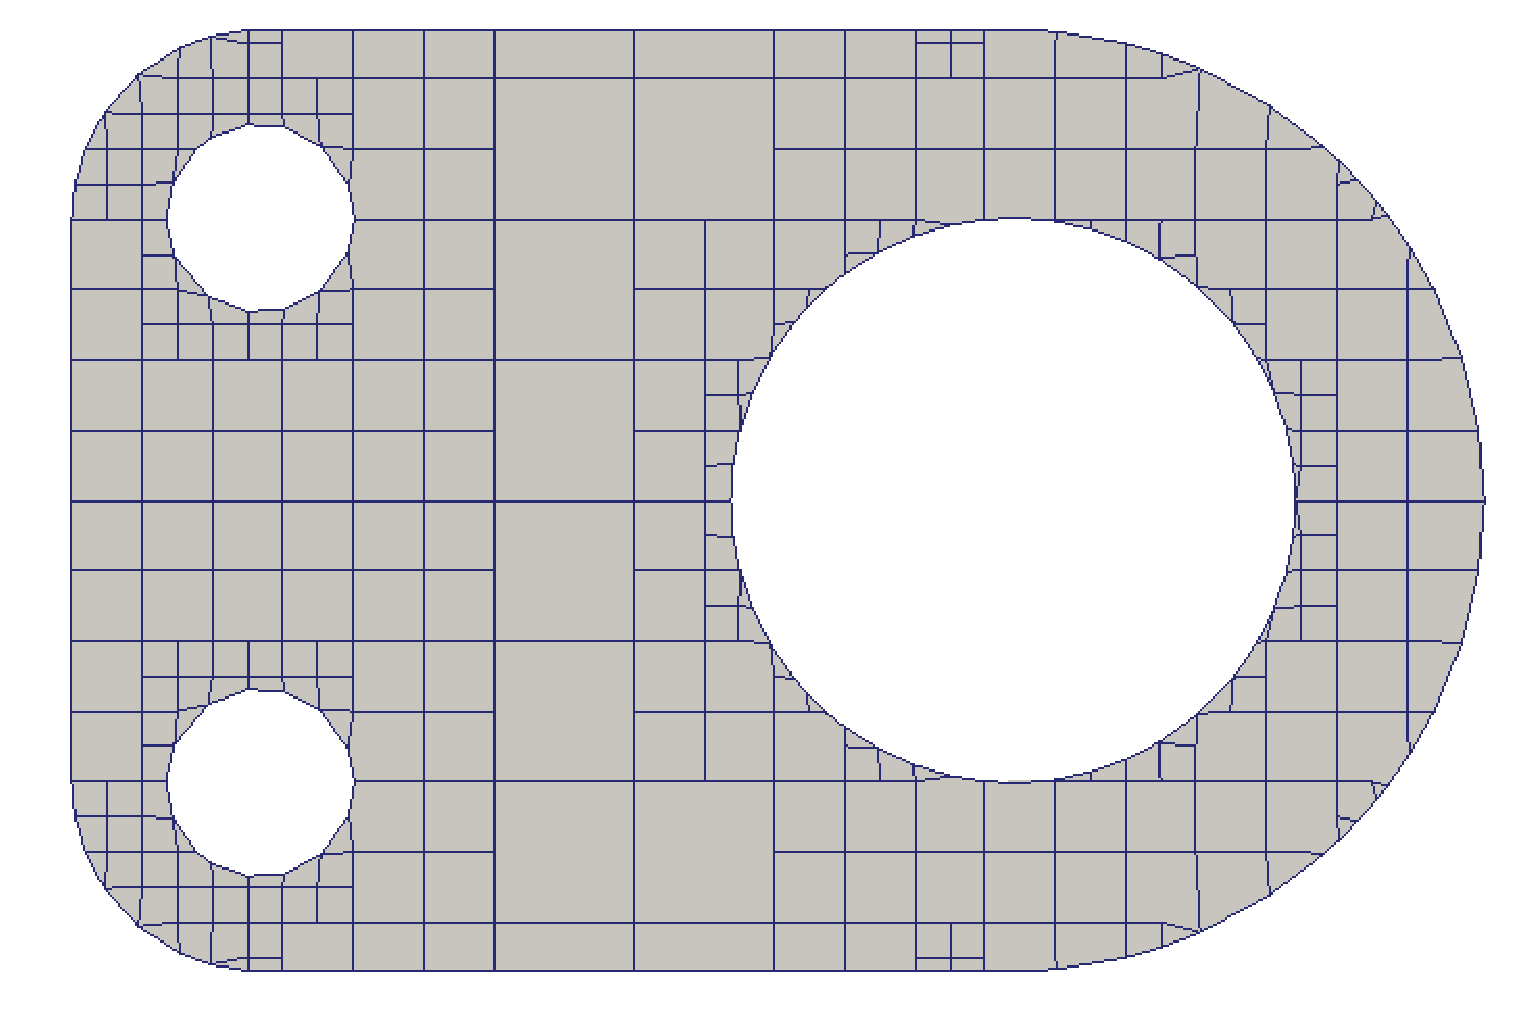
\includegraphics{quadtree/ex_images/ex_bracket_mesh_64_4.eps}
        }
        \caption{Mesh with $res=64$, $s_{max}=4$, 1656 DOFs}
    \end{subfigure}
    \\
    % \begin{subfigure}[b]{1\linewidth}
    %     \centering
    %     \scalebox{0.4}{
    %         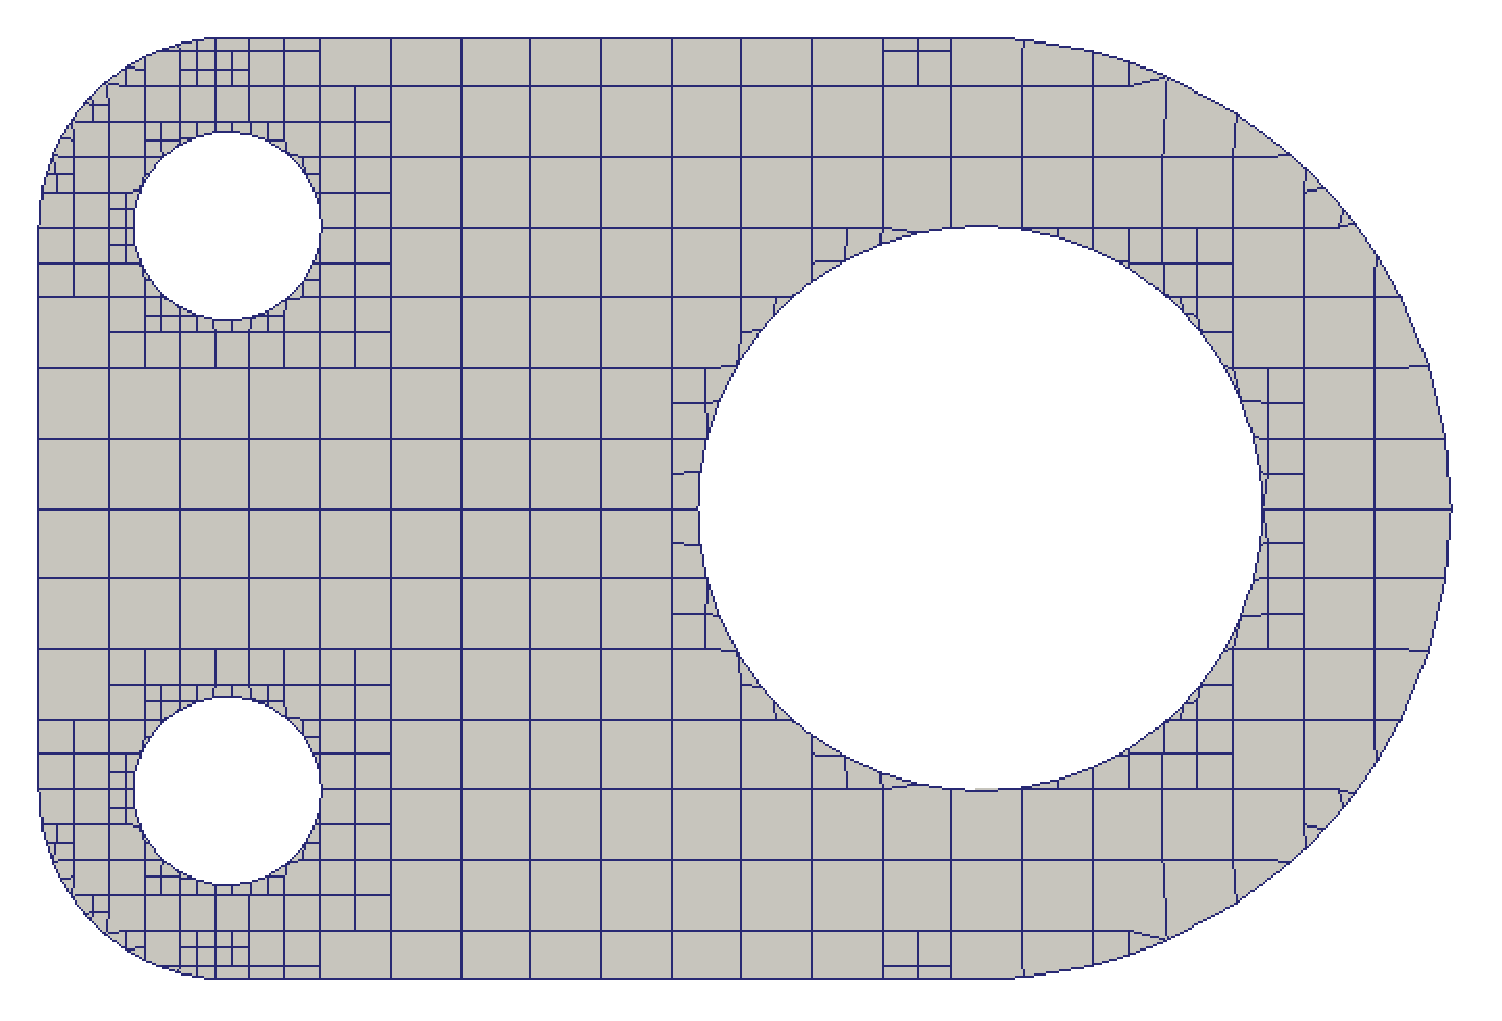
\includegraphics{quadtree/ex_images/ex_bracket_mesh_128_4.eps}
    %     }
    %     \caption{Mesh with $res=128$, $s_{max}=4$, 2548 DOFs}
    % \end{subfigure}
\end{figure}

\begin{figure}[H]\ContinuedFloat
    \begin{subfigure}[b]{1\linewidth}
        \centering
        \scalebox{0.4}{
            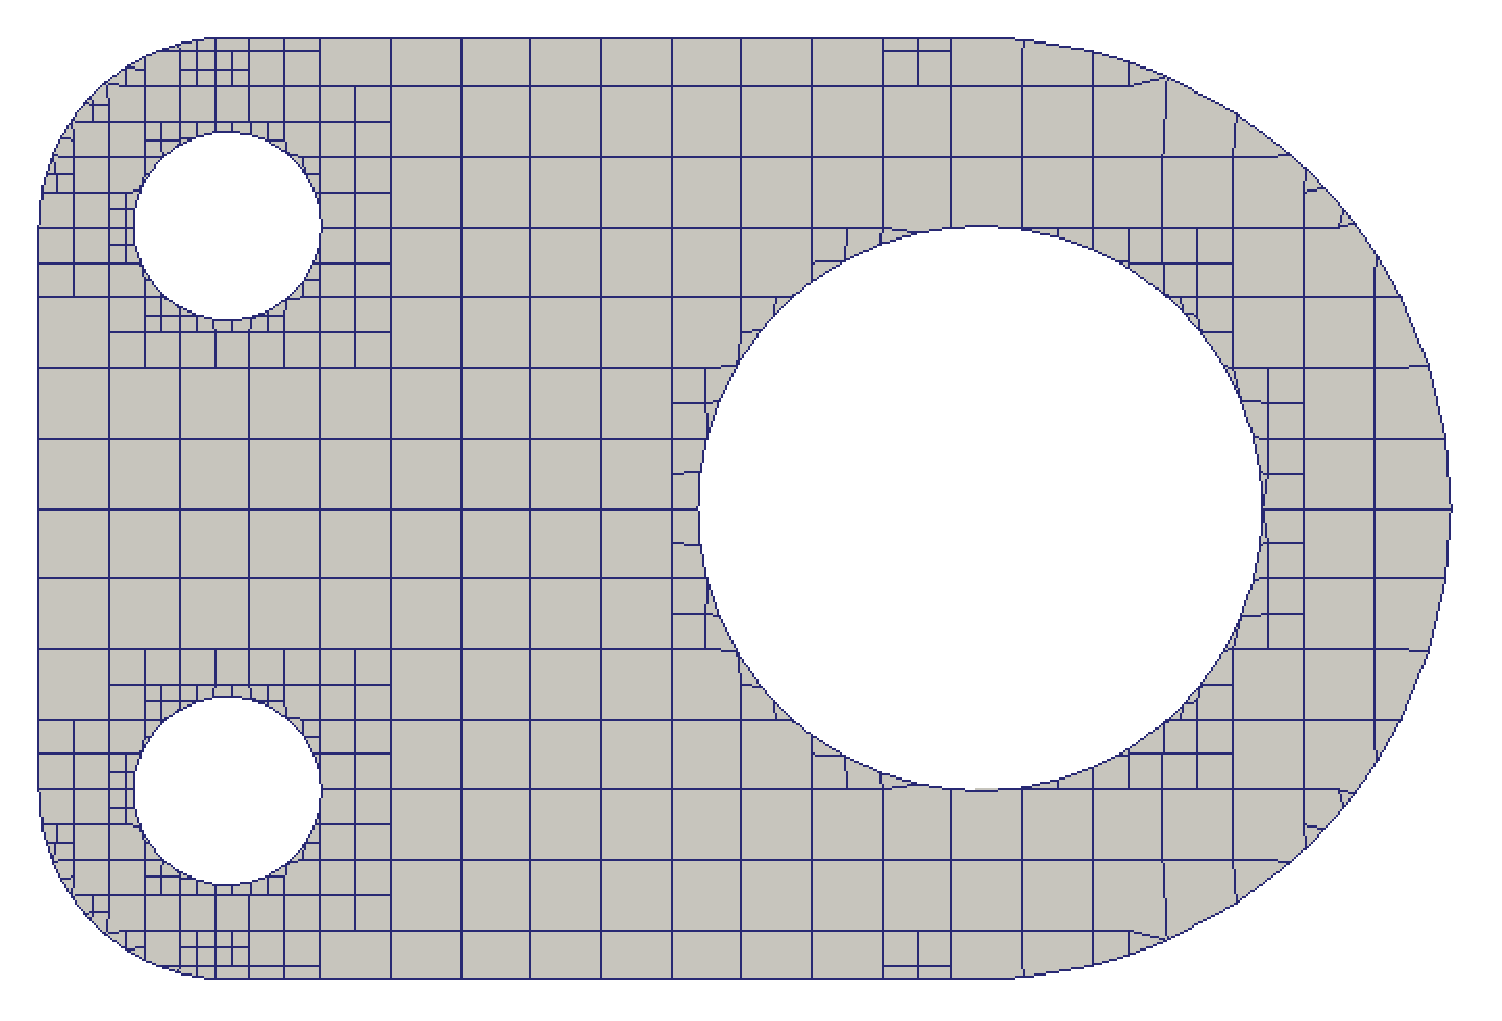
\includegraphics{quadtree/ex_images/ex_bracket_mesh_128_4.eps}
        }
        \caption{Mesh with $res=128$, $s_{max}=4$, 2548 DOFs}
    \end{subfigure}
    \begin{subfigure}[b]{1\linewidth}
        \centering
        \scalebox{0.4}{
            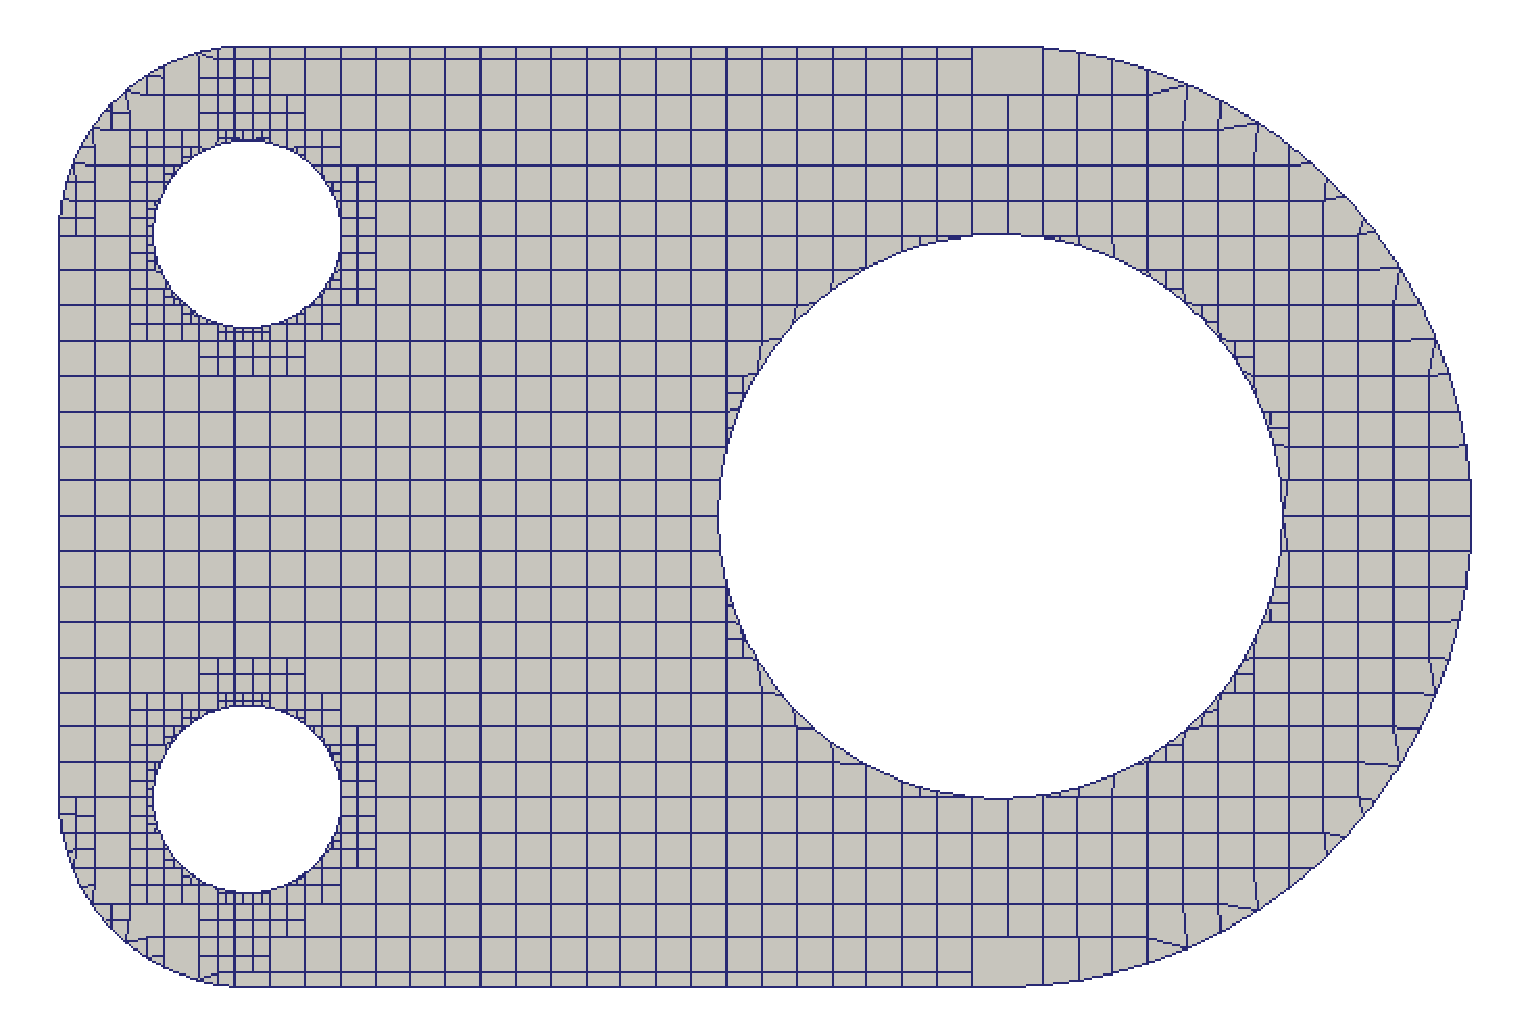
\includegraphics{quadtree/ex_images/ex_bracket_mesh_256_4.eps}
        }
        \caption{Mesh with $res=256$, $s_{max}=4$, 5464 DOFs}
    \end{subfigure}
    \caption[Mesh of the plane strain bracket]{Mesh of the plane strain bracket}
    \label{qdt_fig:ex_bracket_mesh_all}
\end{figure}

\begin{figure}[H]
    \centering
    \scalebox{0.75}{
        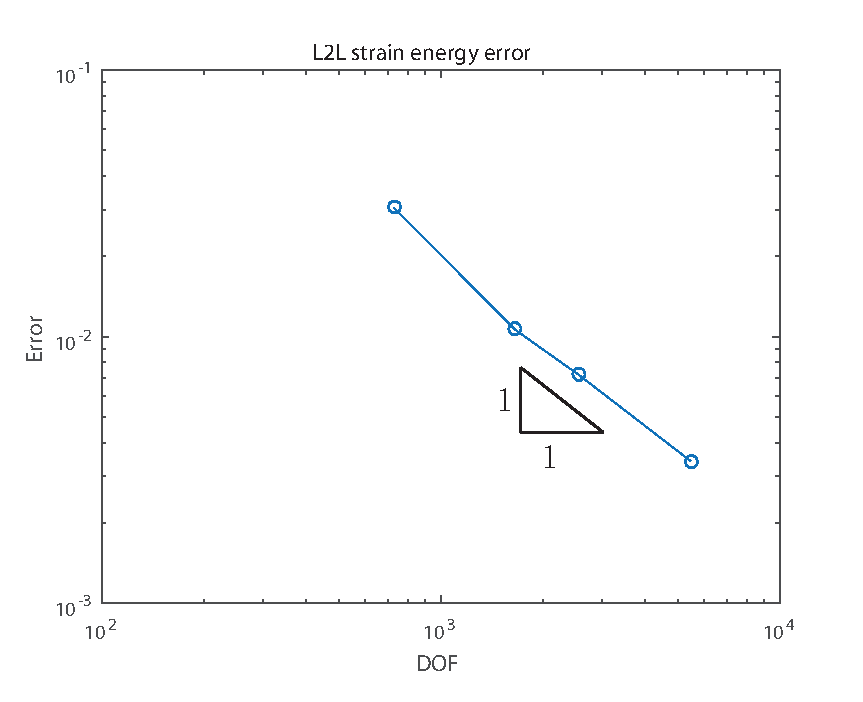
\includegraphics{quadtree/ex_images/ex_bracket_conv.eps}
    }   
    \caption[Convergence of the plane strain bracket]{Convergence of the plane strain bracket}
    \label{qdt_fig:ex_bracket_mesh_conv}
\end{figure}


\paragraph{}
Fig.~\ref{qdt_fig:bracket_stress_contour} shows the von Mises equivalent stress for the plane strain bracket.
From Fig.~\ref{qdt_fig:bracket_stress_contour}, it can be observed that the results from the present approach qualitatively match with the FE solution.
\begin{figure}[h!]
    \begin{subfigure}[b]{1\linewidth}
        \centering
        \scalebox{0.4}{
            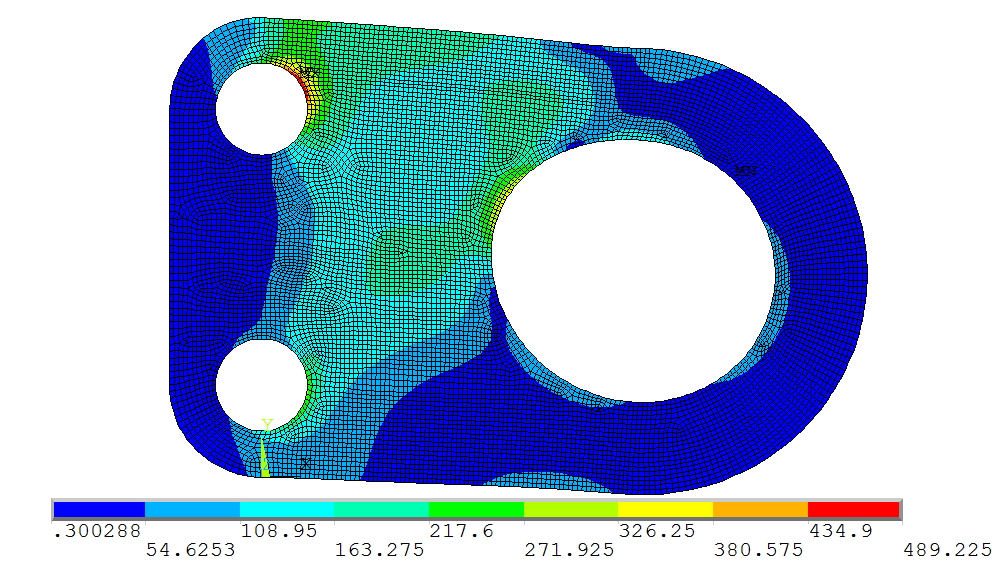
\includegraphics{quadtree/ex_images/ex_bracket_ansys_vmstr.png}
        }
        \caption{FEM}
    \end{subfigure}
    \begin{subfigure}[b]{1\linewidth}
        \centering
        \scalebox{0.4}{
            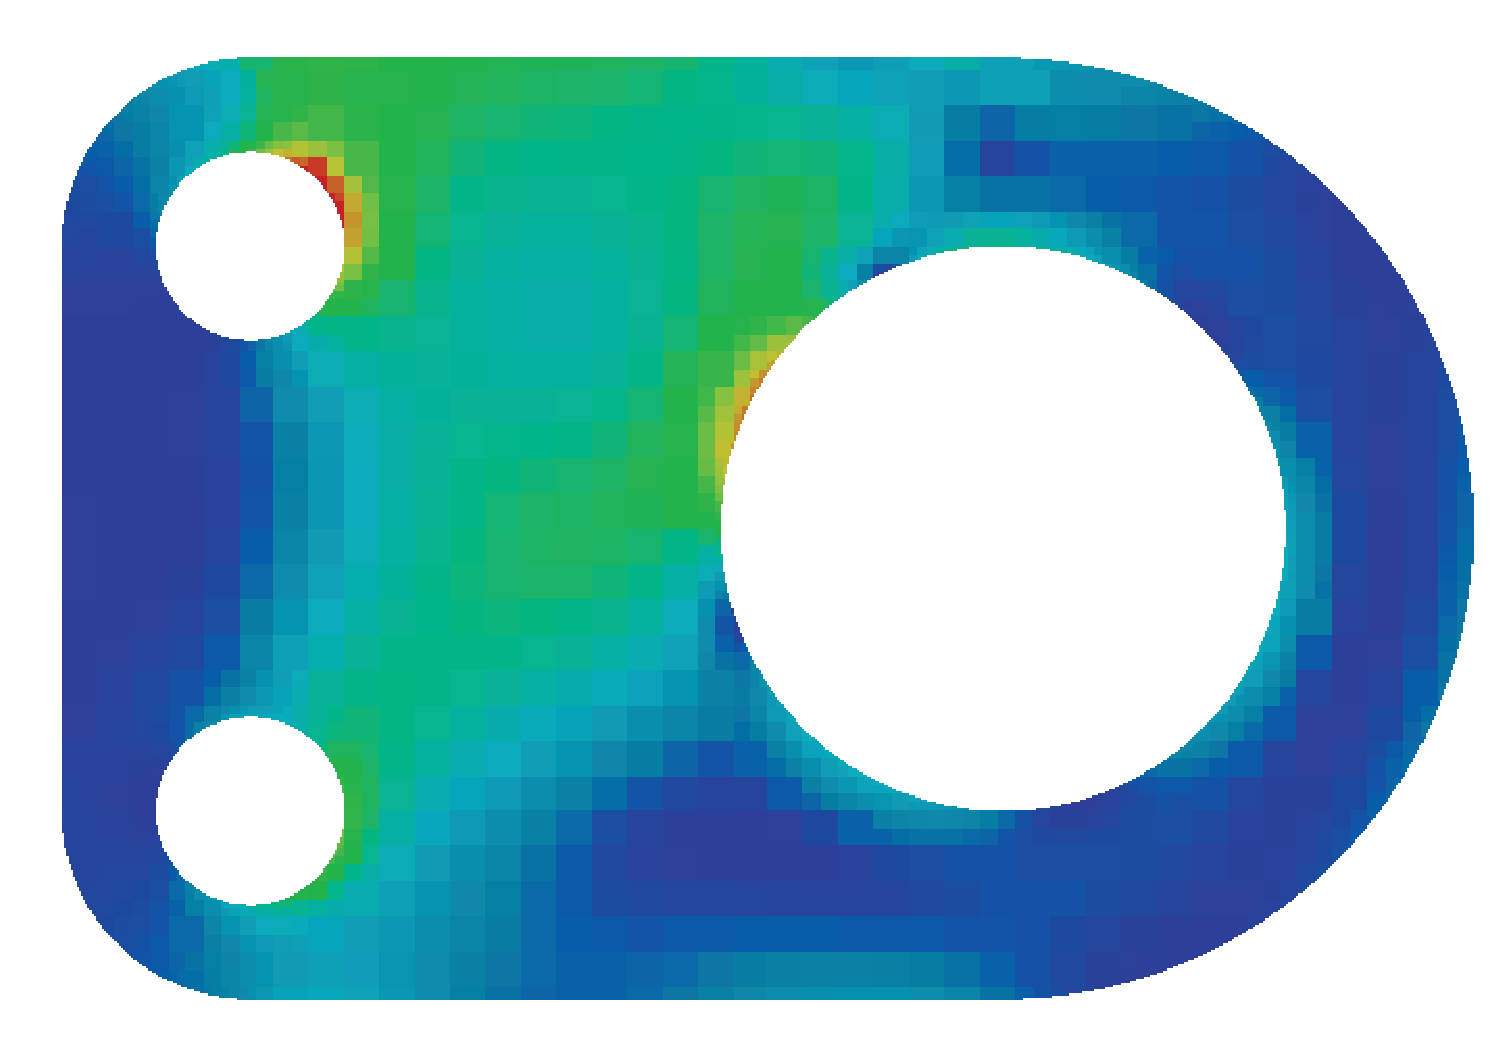
\includegraphics{quadtree/ex_images/ex_bracket_strcontour.eps}
        }
        \caption{Quadtree SBFEM}
    \end{subfigure}

    \caption{Von Mises equivalent stress contours for plane strain bracket}
    \label{qdt_fig:bracket_stress_contour}
\end{figure}